\documentclass[letterpaper,compsoc,twoside]{IEEEtran}
% generated by Docutils <http://docutils.sourceforge.net/>
\usepackage{fixltx2e} % LaTeX patches, \textsubscript
\usepackage{cmap} % fix search and cut-and-paste in Acrobat
\usepackage{ifthen}
\usepackage[T1]{fontenc}
\usepackage[utf8]{inputenc}

\usepackage[font={small,it},labelfont=bf]{caption}
\usepackage{float}

\setcounter{secnumdepth}{0}

%%% Custom LaTeX preamble
\usepackage{scipy}
\makeatletter
\def\PY@reset{\let\PY@it=\relax \let\PY@bf=\relax%
    \let\PY@ul=\relax \let\PY@tc=\relax%
    \let\PY@bc=\relax \let\PY@ff=\relax}
\def\PY@tok#1{\csname PY@tok@#1\endcsname}
\def\PY@toks#1+{\ifx\relax#1\empty\else%
    \PY@tok{#1}\expandafter\PY@toks\fi}
\def\PY@do#1{\PY@bc{\PY@tc{\PY@ul{%
    \PY@it{\PY@bf{\PY@ff{#1}}}}}}}
\def\PY#1#2{\PY@reset\PY@toks#1+\relax+\PY@do{#2}}

\expandafter\def\csname PY@tok@mh\endcsname{\def\PY@tc##1{\textcolor[rgb]{0.13,0.50,0.31}{##1}}}
\expandafter\def\csname PY@tok@s2\endcsname{\def\PY@tc##1{\textcolor[rgb]{0.25,0.44,0.63}{##1}}}
\expandafter\def\csname PY@tok@vc\endcsname{\def\PY@tc##1{\textcolor[rgb]{0.73,0.38,0.84}{##1}}}
\expandafter\def\csname PY@tok@mi\endcsname{\def\PY@tc##1{\textcolor[rgb]{0.13,0.50,0.31}{##1}}}
\expandafter\def\csname PY@tok@ow\endcsname{\let\PY@bf=\textbf\def\PY@tc##1{\textcolor[rgb]{0.00,0.44,0.13}{##1}}}
\expandafter\def\csname PY@tok@c\endcsname{\let\PY@it=\textit\def\PY@tc##1{\textcolor[rgb]{0.25,0.50,0.56}{##1}}}
\expandafter\def\csname PY@tok@ch\endcsname{\let\PY@it=\textit\def\PY@tc##1{\textcolor[rgb]{0.25,0.50,0.56}{##1}}}
\expandafter\def\csname PY@tok@vg\endcsname{\def\PY@tc##1{\textcolor[rgb]{0.73,0.38,0.84}{##1}}}
\expandafter\def\csname PY@tok@cpf\endcsname{\let\PY@it=\textit\def\PY@tc##1{\textcolor[rgb]{0.25,0.50,0.56}{##1}}}
\expandafter\def\csname PY@tok@k\endcsname{\let\PY@bf=\textbf\def\PY@tc##1{\textcolor[rgb]{0.00,0.44,0.13}{##1}}}
\expandafter\def\csname PY@tok@nv\endcsname{\def\PY@tc##1{\textcolor[rgb]{0.73,0.38,0.84}{##1}}}
\expandafter\def\csname PY@tok@no\endcsname{\def\PY@tc##1{\textcolor[rgb]{0.38,0.68,0.84}{##1}}}
\expandafter\def\csname PY@tok@nb\endcsname{\def\PY@tc##1{\textcolor[rgb]{0.00,0.44,0.13}{##1}}}
\expandafter\def\csname PY@tok@gp\endcsname{\let\PY@bf=\textbf\def\PY@tc##1{\textcolor[rgb]{0.78,0.36,0.04}{##1}}}
\expandafter\def\csname PY@tok@na\endcsname{\def\PY@tc##1{\textcolor[rgb]{0.25,0.44,0.63}{##1}}}
\expandafter\def\csname PY@tok@nl\endcsname{\let\PY@bf=\textbf\def\PY@tc##1{\textcolor[rgb]{0.00,0.13,0.44}{##1}}}
\expandafter\def\csname PY@tok@ni\endcsname{\let\PY@bf=\textbf\def\PY@tc##1{\textcolor[rgb]{0.84,0.33,0.22}{##1}}}
\expandafter\def\csname PY@tok@nt\endcsname{\let\PY@bf=\textbf\def\PY@tc##1{\textcolor[rgb]{0.02,0.16,0.45}{##1}}}
\expandafter\def\csname PY@tok@gu\endcsname{\let\PY@bf=\textbf\def\PY@tc##1{\textcolor[rgb]{0.50,0.00,0.50}{##1}}}
\expandafter\def\csname PY@tok@gh\endcsname{\let\PY@bf=\textbf\def\PY@tc##1{\textcolor[rgb]{0.00,0.00,0.50}{##1}}}
\expandafter\def\csname PY@tok@si\endcsname{\let\PY@it=\textit\def\PY@tc##1{\textcolor[rgb]{0.44,0.63,0.82}{##1}}}
\expandafter\def\csname PY@tok@kt\endcsname{\def\PY@tc##1{\textcolor[rgb]{0.56,0.13,0.00}{##1}}}
\expandafter\def\csname PY@tok@sb\endcsname{\def\PY@tc##1{\textcolor[rgb]{0.25,0.44,0.63}{##1}}}
\expandafter\def\csname PY@tok@s\endcsname{\def\PY@tc##1{\textcolor[rgb]{0.25,0.44,0.63}{##1}}}
\expandafter\def\csname PY@tok@mb\endcsname{\def\PY@tc##1{\textcolor[rgb]{0.13,0.50,0.31}{##1}}}
\expandafter\def\csname PY@tok@nc\endcsname{\let\PY@bf=\textbf\def\PY@tc##1{\textcolor[rgb]{0.05,0.52,0.71}{##1}}}
\expandafter\def\csname PY@tok@go\endcsname{\def\PY@tc##1{\textcolor[rgb]{0.20,0.20,0.20}{##1}}}
\expandafter\def\csname PY@tok@gs\endcsname{\let\PY@bf=\textbf}
\expandafter\def\csname PY@tok@mo\endcsname{\def\PY@tc##1{\textcolor[rgb]{0.13,0.50,0.31}{##1}}}
\expandafter\def\csname PY@tok@w\endcsname{\def\PY@tc##1{\textcolor[rgb]{0.73,0.73,0.73}{##1}}}
\expandafter\def\csname PY@tok@ge\endcsname{\let\PY@it=\textit}
\expandafter\def\csname PY@tok@cp\endcsname{\def\PY@tc##1{\textcolor[rgb]{0.00,0.44,0.13}{##1}}}
\expandafter\def\csname PY@tok@ne\endcsname{\def\PY@tc##1{\textcolor[rgb]{0.00,0.44,0.13}{##1}}}
\expandafter\def\csname PY@tok@sh\endcsname{\def\PY@tc##1{\textcolor[rgb]{0.25,0.44,0.63}{##1}}}
\expandafter\def\csname PY@tok@ss\endcsname{\def\PY@tc##1{\textcolor[rgb]{0.32,0.47,0.09}{##1}}}
\expandafter\def\csname PY@tok@il\endcsname{\def\PY@tc##1{\textcolor[rgb]{0.13,0.50,0.31}{##1}}}
\expandafter\def\csname PY@tok@mf\endcsname{\def\PY@tc##1{\textcolor[rgb]{0.13,0.50,0.31}{##1}}}
\expandafter\def\csname PY@tok@sd\endcsname{\let\PY@it=\textit\def\PY@tc##1{\textcolor[rgb]{0.25,0.44,0.63}{##1}}}
\expandafter\def\csname PY@tok@bp\endcsname{\def\PY@tc##1{\textcolor[rgb]{0.00,0.44,0.13}{##1}}}
\expandafter\def\csname PY@tok@gd\endcsname{\def\PY@tc##1{\textcolor[rgb]{0.63,0.00,0.00}{##1}}}
\expandafter\def\csname PY@tok@gi\endcsname{\def\PY@tc##1{\textcolor[rgb]{0.00,0.63,0.00}{##1}}}
\expandafter\def\csname PY@tok@kn\endcsname{\let\PY@bf=\textbf\def\PY@tc##1{\textcolor[rgb]{0.00,0.44,0.13}{##1}}}
\expandafter\def\csname PY@tok@nf\endcsname{\def\PY@tc##1{\textcolor[rgb]{0.02,0.16,0.49}{##1}}}
\expandafter\def\csname PY@tok@sr\endcsname{\def\PY@tc##1{\textcolor[rgb]{0.14,0.33,0.53}{##1}}}
\expandafter\def\csname PY@tok@vi\endcsname{\def\PY@tc##1{\textcolor[rgb]{0.73,0.38,0.84}{##1}}}
\expandafter\def\csname PY@tok@nn\endcsname{\let\PY@bf=\textbf\def\PY@tc##1{\textcolor[rgb]{0.05,0.52,0.71}{##1}}}
\expandafter\def\csname PY@tok@o\endcsname{\def\PY@tc##1{\textcolor[rgb]{0.40,0.40,0.40}{##1}}}
\expandafter\def\csname PY@tok@err\endcsname{\def\PY@bc##1{\setlength{\fboxsep}{0pt}\fcolorbox[rgb]{1.00,0.00,0.00}{1,1,1}{\strut ##1}}}
\expandafter\def\csname PY@tok@nd\endcsname{\let\PY@bf=\textbf\def\PY@tc##1{\textcolor[rgb]{0.33,0.33,0.33}{##1}}}
\expandafter\def\csname PY@tok@sx\endcsname{\def\PY@tc##1{\textcolor[rgb]{0.78,0.36,0.04}{##1}}}
\expandafter\def\csname PY@tok@cs\endcsname{\def\PY@tc##1{\textcolor[rgb]{0.25,0.50,0.56}{##1}}\def\PY@bc##1{\setlength{\fboxsep}{0pt}\colorbox[rgb]{1.00,0.94,0.94}{\strut ##1}}}
\expandafter\def\csname PY@tok@kr\endcsname{\let\PY@bf=\textbf\def\PY@tc##1{\textcolor[rgb]{0.00,0.44,0.13}{##1}}}
\expandafter\def\csname PY@tok@m\endcsname{\def\PY@tc##1{\textcolor[rgb]{0.13,0.50,0.31}{##1}}}
\expandafter\def\csname PY@tok@kc\endcsname{\let\PY@bf=\textbf\def\PY@tc##1{\textcolor[rgb]{0.00,0.44,0.13}{##1}}}
\expandafter\def\csname PY@tok@cm\endcsname{\let\PY@it=\textit\def\PY@tc##1{\textcolor[rgb]{0.25,0.50,0.56}{##1}}}
\expandafter\def\csname PY@tok@gt\endcsname{\def\PY@tc##1{\textcolor[rgb]{0.00,0.27,0.87}{##1}}}
\expandafter\def\csname PY@tok@kp\endcsname{\def\PY@tc##1{\textcolor[rgb]{0.00,0.44,0.13}{##1}}}
\expandafter\def\csname PY@tok@kd\endcsname{\let\PY@bf=\textbf\def\PY@tc##1{\textcolor[rgb]{0.00,0.44,0.13}{##1}}}
\expandafter\def\csname PY@tok@gr\endcsname{\def\PY@tc##1{\textcolor[rgb]{1.00,0.00,0.00}{##1}}}
\expandafter\def\csname PY@tok@s1\endcsname{\def\PY@tc##1{\textcolor[rgb]{0.25,0.44,0.63}{##1}}}
\expandafter\def\csname PY@tok@se\endcsname{\let\PY@bf=\textbf\def\PY@tc##1{\textcolor[rgb]{0.25,0.44,0.63}{##1}}}
\expandafter\def\csname PY@tok@sc\endcsname{\def\PY@tc##1{\textcolor[rgb]{0.25,0.44,0.63}{##1}}}
\expandafter\def\csname PY@tok@c1\endcsname{\let\PY@it=\textit\def\PY@tc##1{\textcolor[rgb]{0.25,0.50,0.56}{##1}}}

\def\PYZbs{\char`\\}
\def\PYZus{\char`\_}
\def\PYZob{\char`\{}
\def\PYZcb{\char`\}}
\def\PYZca{\char`\^}
\def\PYZam{\char`\&}
\def\PYZlt{\char`\<}
\def\PYZgt{\char`\>}
\def\PYZsh{\char`\#}
\def\PYZpc{\char`\%}
\def\PYZdl{\char`\$}
\def\PYZhy{\char`\-}
\def\PYZsq{\char`\'}
\def\PYZdq{\char`\"}
\def\PYZti{\char`\~}
% for compatibility with earlier versions
\def\PYZat{@}
\def\PYZlb{[}
\def\PYZrb{]}
\makeatother


%%% User specified packages and stylesheets

%%% Fallback definitions for Docutils-specific commands

% hyperlinks:
\ifthenelse{\isundefined{\hypersetup}}{
  \usepackage[colorlinks=true,linkcolor=blue,urlcolor=blue]{hyperref}
  \urlstyle{same} % normal text font (alternatives: tt, rm, sf)
}{}


%%% Body
\begin{document}
\newcounter{footnotecounter}\title{ObjArray: Better Integrating Python Objects with NumPy Arrays}\author{Justin C. Fisher$^{\setcounter{footnotecounter}{3}\fnsymbol{footnotecounter}\setcounter{footnotecounter}{1}\fnsymbol{footnotecounter}}$%
          \setcounter{footnotecounter}{1}\thanks{\fnsymbol{footnotecounter} %
          Corresponding author: \protect\href{mailto:fisher@smu.edu}{fisher@smu.edu}}\setcounter{footnotecounter}{3}\thanks{\fnsymbol{footnotecounter} Southern Methodist University, Department of Philosophy}\thanks{%

          \noindent%
          Copyright\,\copyright\,2010 Justin C. Fisher. This is an open-access article distributed under the terms of the Creative Commons Attribution License, which permits unrestricted use, distribution, and reproduction in any medium, provided the original author and source are credited.%
        }}\maketitle
          \renewcommand{\leftmark}{PROC. OF THE 9th PYTHON IN SCIENCE CONF. (SCIPY 2010)}
          \renewcommand{\rightmark}{OBJARRAY: BETTER INTEGRATING PYTHON OBJECTS WITH NUMPY ARRAYS}
        



\InputIfFileExists{page_numbers.tex}{}{}
\newcommand*{\docutilsroleref}{\ref}
\newcommand*{\docutilsrolelabel}{\label}
\providecommand*\DUrolecite[1]{\cite{#1}}
\begin{abstract}There are many well-known benefits of Object Oriented Programming (OOP), including allowing hierarchically classed objects to possess and inherit diverse attributes and methods.  There are also well-known benefits of Numeric Python (NumPy) arrays, including speed, a vast library of powerful functions, and flexible indexing.  Before now, it was quite cumbersome for Python coders to enjoy both sorts of benefits at the same time.  Python's objects offer excellent OOP, but could not easily be used with NumPy.  NumPy's structured record arrays offer NumPy virtues but only a pale approximation of OOP.  NumPy also allows arrays of Python objects, but these provide only fancy indexing, not straightforward access to OOP attributes or methods, nor direct access to the vast library of fast NumPy functions.  Instead, coders who want to enjoy both OOP and NumPy have needed to write many explicit loops/mappings/comprehensions to copy arrayed objects' attributes into NumPy arrays and vice versa.  My free package, ObjArray, offers a solution to this problem, providing NumPy users clean natural access to OOP attributes and methods-{}-for example, \texttt{people{[} people.age > 18 {]}.height} does exactly what you would intuitively expect it should do, namely return a NumPy array of the height attributes of all the people over age 18-{}-all while providing full access to the speed, power, and flexible indexing of NumPy.\end{abstract}\begin{IEEEkeywords}Python, NumPy, Object-Oriented, Object, Array, Vectorized\end{IEEEkeywords}

\subsection{1.  Goals.%
  \label{goals}%
}


The overall goal of my free package ObjArray is to better integrate Python's object-oriented programming (OOP) features with Numeric Python (NumPy).  Such integration would be suitable for some, but not all, Python projects.  Python's OOP may not be suitable for projects involving extremely large data sets because Python's objects are not especially efficient in terms of memory storage or processing speed.  Conversely, very small Python projects may have little need for NumPy's speed (though other features may still be useful).  Very many Python projects fall between these extremes.  These \textquotedbl{}medium-sized\textquotedbl{} projects are large enough to need, in some places, to draw upon fast powerful NumPy functions, but are small enough that memory considerations permit using numerous Python objects and speed considerations allow that many non-time-sensitive operations can be written in an OOP format that is often easier for many coders to write, read, understand, and debug.  These medium-sized projects could be well served by a package like ObjArray that makes it much simpler to take full advantage of the strengths of both OOP and NumPy.

\subsubsection{1.1. Object-Oriented Goals.%
  \label{object-oriented-goals}%
}
\begin{quotation}%
\begin{quote}


\textbf{O1.  Familiar Python objects in familiar class hierarchies.} A good integration of Python OOP and NumPy should make it easy to take code that began as pure Python OOP and to expose the attributes of arrayed Python objects for use in fast NumPy functions.  In particular, we'd want object arrays to contain familiar Python objects, situated in familiar class hierarchies.  For example, if A is a list, tuple, or array of ordinary Python objects, a simple command like \texttt{OA = ObjArray( A )} should suffice to create an array of those objects with easy access to the other features listed below.

\textbf{O2.  Flexible object size.}  Different objects in the same class may contain data of different sizes (e.g., strings of different lengths), and some may possess attributes or methods that others lack.  This flexibility is a distinguishing feature of Python's OOP and is appreciated by many coders.  NumPy itself does not generally allow this sort of flexibility, but our integration of OOP with NumPy should.

\textbf{O3.  Attributes of arrayed objects should be easily accessible by familiar dot idiom.}  If \texttt{Adam} is an individual object, then all Python coders know that \texttt{Adam.height} probably returns Adam's height attribute.  We should support parallel behavior for arrays of objects.  For example, if \texttt{people} is an array of person objects, then \texttt{people.height} should return an array the same shape as \texttt{people}, containing each person's \texttt{.height} attribute.

\textbf{O4.  Methods of arrayed objects should be easily callable by familiar dot idiom.}  Similarly, for individual objects, we all know that \texttt{Adam.grow(1)} will call Adam's \texttt{.grow} method, with Adam being passed in as an implicit \textquotedbl{}self\textquotedbl{} argument, and 1 being passed as the explicit argument.  We should support parallel behavior for arrays of objects, so \texttt{people.grow(1)} should call each person's grow method on herself with argument 1, and \texttt{people.grow(people.height)} should call each person's grow method on herself with her own height as the argument.
\end{quote}
\end{quotation}

Python nicely provides these four OOP features for individual objects, but does not offer them collectively for objects organized into arrays.  Instead, coders who want to use OOP features for arrayed objects typically must write explicit loops to deal with the objects one at a time.  It would be better if OOP could also achieve some of the goals NumPy accomplishes by allowing fast and powerful \textquotedbl{}vectorized\textquotedbl{} operations to operate upon many arrayed items at once.

\subsubsection{1.2.  NumPy Goals.%
  \label{numpy-goals}%
}
\begin{quotation}%
\begin{quote}


\textbf{N1.  Speed.}  Interpreted Python code is often notoriously slow, whereas NumPy allows for comparatively fast operations over whole arrays at once.  A good integration of Python OOP with NumPy must easily allow for full speed NumPy operations involving the attributes of arrayed objects.  For example, \texttt{people.height.mean()} should use NumPy's \texttt{mean} function to average the arrayed people's heights.

\textbf{N2.  Huge library of powerful functions.}  There exist many powerful and freely available functions that operate on NumPy arrays, including functions in NumPy, SciPy, and other packages.  A good integration of OOP and NumPy should make it easy to expose arrayed objects' attributes to many of these existing functions.

\textbf{N3.  Vectorized operations, notation and broadcasting.}  NumPy allows coders to use very concise code to execute vectorized operations that act upon many array elements at once without the coder needing to write any explicit looping, nor even to pay much ongoing attention to the internal structure of the arrays.  For example, \texttt{A1 > (A2 * 1.3)} yields a Boolean array with the same shape as arrays A1 and A2 (when broadcast together), which is True wherever the stated inequality holds between corresponding elements of these arrays, something that many languages would require be written with explicit loops, yielding tediously convoluted code at best and hard-to-notice bugs at worst.  We should allow a similar level of crisp clean abstraction for operations involving object attributes.  For example, \texttt{obese = people.weight > (people.height * 1.3)} should also produce a Boolean array.  In addition, such concise vectorized notation should automatically broadcast compatible arrays in the ways NumPy users intuitively expect.  For example, in the above calculations the scalar 1.3 is broadcast to match the shape of the arrays.  This concise notation and broadcasting should apply not just for attributes of arrayed objects (as in O3 above), but also for vectorized method calls (as in O4).

\textbf{N4.  Indexing and Slicing.}  Any good integration of OOP and NumPy must allow full use of NumPy's excellent slicing and indexing tools.  It should also allow for object attributes to easily play a role in the criteria for \textquotedbl{}fancy indexing\textquotedbl{}.  So, for example, \texttt{people{[} people.age > 18 {]}} should generate a new array containing just those people whose age attribute is greater than 18.
\end{quote}
\end{quotation}

\subsection{2.  Existing ways of integrating Python OOP with NumPy.%
  \label{existing-ways-of-integrating-python-oop-with-numpy}%
}


NumPy currently offers two partial ways of integrating NumPy arrays with OOP: record arrays and arrays with dtype=object.  Both fall short of the goals laid out above, but the shortcomings of the second can be overcome, in part by drawing a key insight from the first.

\subsubsection{2.1.  NumPy's Record Arrays.%
  \label{numpy-s-record-arrays}%
}


NumPy's record arrays (aka \textquotedbl{}structured arrays\textquotedbl{}) allow fancy indexing and full participation in the vast library of fast NumPy functions (N1-N4).  Sadly, record arrays fall short of our object-oriented goals:\begin{quotation}%
\begin{quote}


\textbf{O1.}  Record arrays do not contain familiar Python objects, but instead what I will call \textquotedbl{}record-objects\textquotedbl{}, a new sort of entity that provides a pale approximation of some OOP features.  Record-objects do not participate in class hierarchies in the ways that OOP coders would expect.

\textbf{O2.}  Each record array must pre-declare a finite list of attributes that the arrayed record-objects will all possess, each with a fixed size in bytes.  This forbids the flexible object-sizing that many Python programmers expect.

\textbf{O3.}  Record arrays use idiosyncratic string indexing to access attributes of arrayed record-objects.  For example, you would retrieve an array of people's heights with \texttt{people{[}'height'{]}}.  It would be preferable instead to use the familiar OOP dot idiom: \texttt{people.height}.

\textbf{O4.}  Record arrays provide no straightforward means to write or call methods for particular record-objects, nor any straightforward way to call the same method for all arrayed objects.
\end{quote}
\end{quotation}

One might hope that we could somehow \textquotedbl{}soup up\textquotedbl{} record-objects to make them better able to provide OOP features like those of Python objects.  Even if we did manage to reinvent the wheel in this way, we would still end up in the awkward circumstance of having two \textquotedbl{}separate but not quite equal\textquotedbl{} forms of OOP available to Python coders:  original Python objects and whatever souped-up version of record-objects we come up with.  The present paper and my ObjArray package instead aim to provide an easy interface between familiar Python objects and fast NumPy operations, not to make coders learn to use some new sort of \textquotedbl{}record-object\textquotedbl{} that mimics some OOP features.  So, record arrays will not be of much direct use to us.  There is however some value to the idea that we might want some attribute values of arrayed objects to be permanently stored together in a NumPy array, an idea revisited in Section 4.

\subsubsection{2.2.  NumPy arrays with dtype=object.%
  \label{numpy-arrays-with-dtype-object}%
}


NumPy offers a second partial integration of NumPy arrays with Python objects.  Most NumPy arrays have a numerical dtype, like integer or float, and store numerical values together in a block of memory.  However, NumPy arrays with dtype=object instead store pointers to ordinary Python objects, and when an individual element of such an array is accessed, the pointed-to object is returned.  These arrays provide a smattering of OOP and NumPy benefits, but don't fully deliver in either category.\begin{quotation}%
\begin{quote}


\textbf{O1 and O2.}  Happily, these arrayed objects are ordinary Python objects (not the pale \textquotedbl{}record-objects\textquotedbl{} employed by record arrays) so they display the familiar class hierarchy and flexible sizing that we expect of Python objects.

\textbf{O3.}  Sadly, there is no simple way to produce an array containing a given attribute of the arrayed objects.  Instead coders need to explicitly copy attribute values into arrays when they want to use NumPy-{}-e.g., using something like \texttt{oldheights = np.array( {[}person.height for person in people{]} )}-{}-and then explicitly copy new attribute values back into objects when they want to use OOP again-{}-e.g.,  using \texttt{for person,newheight in zip(people, newheights): person.height = newheight}.  Of course, things get even more convoluted for arrays with multiple dimensions that the coder somehow needs to iterate over.  It would be preferable to forego the explicit looping, and just use \texttt{oldheights = people.height}, and \texttt{people.height = newheights}.

\textbf{O4.}  Sadly, there also is no simple way to call methods of arrayed objects.  Coders end up again needing to loop explicitly over the objects or to construct custom vectorized \textquotedbl{}ufuncs\textquotedbl{}.  Neither of these options comes anywhere near the beautiful simplicity of \texttt{people.grow(1)}.

\textbf{N1, N2 and N3.}  Sadly, extremely few NumPy functions work when dtype=object.  Instead, one typically must first explicitly construct new arrays with numerical dtypes, as in O3.

\textbf{N4.}  Happily, NumPy's slicing and indexing generally ignore the dtype of array elements, so can be used on arrays of dtype=object.  Sadly though, there is no straightforward way to use object attributes as a criterion in \textquotedbl{}fancy indexing\textquotedbl{}, without again using explicit loops as in O3.
\end{quote}
\end{quotation}

Pessimists might view the preceding as a \textquotedbl{}glass half empty.\textquotedbl{}  NumPy arrays with dtype=object lack many features we expect from NumPy arrays, and force us to write numerous tedious loops to copy values out of arrayed objects into \textquotedbl{}real\textquotedbl{} NumPy arrays when we want to do fast NumPy operations and then to copy updated values back into objects when we want to do OOP again.  This \textquotedbl{}half empty\textquotedbl{} feeling leads many seasoned NumPy coders to eschew object arrays and the comforts of OOP, and instead to settle for the austere efficiency of forcing everything into numerical arrays as much as possible.

I instead see this as a \textquotedbl{}glass half full.\textquotedbl{}  Arrays with dtype=object at least give us arrays of ordinary Python objects with their class hierarchy (O1) and highly flexible internal structure (O2).  They also give us flexible NumPy slicing (N4).  The main ways this solution falls short involve the clumsy explicit loops that coders must use (O4) to call methods of all arrayed objects, and (O3) to copy objects' attribute values to and from arrays whenever they want to switch between fast NumPy operations and convenient OOP.  Fortunately, many of these clumsy explicit loops do the very same things, so it is quite straightforward to automate them.  And part of the diabolical genius of Python is that it allows \textquotedbl{}magic methods\textquotedbl{} that hide heavy-duty automation behind innocuous-looking syntax.  So really, all we need to make our \textquotedbl{}glass almost entirely full\textquotedbl{} is just to create magic methods that provide clean, intuitive syntax for doing the same things that all these explicit loops were doing.  (Better still, we could also figure out ways to minimize how often such automated operations actually will need to loop through and copy a lot of data-{}-more on that in section 4.)

\subsection{3.  Ad Hoc Transfers and Method Calling.%
  \label{ad-hoc-transfers-and-method-calling}%
}


Drawing upon the optimistic \textquotedbl{}glass half full\textquotedbl{} perspective from the preceding section, my ObjArray package employs NumPy arrays with dtype=object.  ObjArrays will typically be created by \texttt{OA = ObjArray(A)}, where A can be any list, tuple, or array of Python objects.  This returns a view of A as a NumPy ndarray of subclass ObjArray and dtype=object.

ObjArray employs various \textquotedbl{}magic methods\textquotedbl{} to enable clean intuitive access to the attributes and methods of arrayed objects.  This access comes in two forms.  Ad hoc methods (discussed in this section) iterate through an ObjArray doing something appropriate with each object, in much the same manner as the explicit loops described in section 2.2.  Since such looping is relatively slow (on NumPy timescales), ad hoc methods are best used in moderation-{}-e.g., once to copy attribute values of arrayed objects into one or more NumPy arrays upon which to perform a batch of intensive calculations, and once again to copy values from an output array back to the attribute values of Python objects.  Coupled buffers (described in Section 4) allow us to dispense with much of this repeated copying back-and-forth, but lack some flexibility of ad hoc methods.

\subsubsection{3.1. Ad Hoc reading.%
  \label{ad-hoc-reading}%
}


Ad hoc reading aims to meet goal O3: reading the values of a particular attribute of arrayed objects and packaging these together into an array that can participate in fast NumPy operations.  For example, this will allow \texttt{people.height} to yield an array with the same shape as \texttt{people}, each of whose elements is the \texttt{.height} attribute of the corresponding person.

To allow this, the class ObjArray has a special \texttt{\_\_get\_\_} method that catches all failed attempts to retrieve an attribute from an ObjArray itself, and instead redirects those attempts to retrieve that attribute from the various objects in the ObjArray and to package those attribute values together in a new array.  If OA is an ObjArray, then \texttt{values = OA.x} will return a new array whose initial dimensions match OA and whose contents match the corresponding \texttt{.x} attribute-instances for the objects in OA, including whatever dimensions those instances have.  For example, if OA is a 5x5 ObjArray, and each \texttt{.x} instance is a 3x3 array of integers, then \texttt{OA.x} would return a 5x5x3x3 array of integers.   The shape and dtype of attribute instances is automatically determined by sampling a member of OA, or you can manually specify these with keyword arguments, via the more verbose \texttt{OA.read\_attr(attr\_name, shape=None, dtype=None)}.

Ad hoc read operations support slicing in two ways.  First, you can slice OA itself before reading, e.g., \texttt{values = OA{[}0:2{]}.x}.  Since a slice of an ObjArray is another ObjArray, slices support ad hoc reading too.   Second you can slice the array produced by ad hoc reading, e.g., \texttt{values = OA.x{[}0:2{]}}.  The former way is often preferable because it reduces the number of items that ad hoc reading must loop through, but only the latter way allows you to slice into the internal structure of attribute instances if they are arrays themselves.  In principle, you could use both ways of slicing in rapid succession, so long as you pay careful attention to the shapes of the two arrays you'll be slicing.

\subsubsection{3.2.  Ad hoc writing.%
  \label{ad-hoc-writing}%
}


\texttt{OA.x = newvalues} is the converse ad hoc write operation.  It broadcasts newvalues to match the shape of OA, and then stores those values as the \texttt{.x} attribute instances of the corresponding objects of OA.  For example, \texttt{people.height = 50} would set everyone's height to 50, and \texttt{people.height = people.height+1} combines ad hoc reading of old heights and ad hoc writing of new incremented heights (or \texttt{people.height += 1} works fine too).

Unfortunately, the Python language forces writing to be more complicated than reading.  For ad hoc reading, I define a blanket \texttt{\_\_get\_\_} method that triggers only upon a failed attempt to retrieve any attribute from OA itself.  This allows attempts to read ordinary attributes of arrays, like OA.shape, to happen at full speed.  Unfortunately Python has no parallel blanket \texttt{\_\_set\_\_} method that triggers only in cases where an attribute does not already exist.  We could override ObjArray's \texttt{\_\_set\_\_} method, but doing so would slightly slow \emph{all} attempts to set an ObjArray's own attributes, including its NumPy attributes.  For most purposes, this slowdown might be negligible, especially because arrays with dtype=object usually don't participate in many time-sensitive operations anyway.  Even if we opted to embrace this slowdown, it still would be difficult to distinguish attempts to set a new attribute of the ObjArray itself from attempts to set a new attribute of the arrayed objects.

For these reasons, I regretfully opted to make the dot idiom for ad hoc writing require some form of prior declaration that an attribute name is to be treated as a writeable attribute of arrayed objects, rather than as a writeable attribute of the ObjArray itself.  This prior declaration can be done explicitly, but more often is implicit-{}-e.g., ad hoc reading an attribute implicitly declares it to be eligible for later writing.  Explicit and implicit declarations both cause a factory to create a new property for the class ObjArray (or for whatever subclass of this you create and employ) whose \texttt{\_\_set\_\_} method intercepts attempts to set \texttt{OA.x} and redirects and broadcasts these to the \texttt{.x} attributes of the arrayed objects (except when \texttt{OA.\_\_dict\_\_} already contains an entry for 'x', in which case that is modified).  In cases where the dot idiom is unavailable-{}-because an attribute hasn't been declared yet, or because the attribute name is one like 'shape' for which NumPy has already dictated a meaning-{}-you can always use the more verbose \texttt{OA.write\_attr('shape')}.

\subsubsection{3.3.  Ad hoc method calling.%
  \label{ad-hoc-method-calling}%
}


A third type of ObjArray ad hoc operation allows you to use a single command to call a method of each arrayed object with NumPy-style broadcasting of arguments (goal O4).  This allows \texttt{people.grow(1)} to call each person's \texttt{.grow} method with the argument 1 automatically broadcast across the array, and it allows \texttt{people.grow( people.height )} to call each person's \texttt{.grow} method with her own \texttt{.height} as the argument.  The outputs returned by the called methods are collected together in an array and returned.  This allows for crisp, clean, easy-to-debug code (satisfying goal N3).

\subsection{4.  Coupled Buffers.%
  \label{coupled-buffers}%
}


The above ad hoc operations are fairly slow by NumPy standards, because each must iterate through all objects in an ObjArray.  This slowdown will likely be minor in comparison to OOP Python operations done on many objects.  However, in cases where you frequently want to access and update information from both object-side and array-side, a coupled buffer can provide much better performance.

Coupled buffers imitate the best feature of NumPy's record arrays (section 2.1), namely the idea of permanently storing the attribute values for arrayed objects together in an array themselves, where they'll always be ready to participate in fast NumPy operations, with no need ever to loop through all the objects themselves to copy their attributes to or from the array.  Record arrays used this arrangement for \emph{all} attributes of the record-objects, which forced these objects to have only a pre-specified number of attributes with pre-specified byte-size, and thereby violated (O4) our desire for flexible object-size.  My coupled buffers avoid this forced rigidity by coupling only select attributes, which allows that objects may possess other (uncoupled) attributes of varying size, and that some objects in an array may possess (uncoupled) attributes that others lack.

The easiest way to create a coupled buffer is with \texttt{B = OA.new\_coupled\_buffer( 'x' )}.  This creates a new \textquotedbl{}buffer\textquotedbl{} array by a process much like ad hoc reading, copying each object's \texttt{.x} attribute value into the corresponding part of the buffer.  Then each object's attribute instance is effectively replaced with a view of the appropriate part of the buffer.  The result is that any subsequent changes to an object's \texttt{.x} attribute will automatically update the coupled portion of the buffer, and conversely any changes in the buffer will automatically be accessible from the corresponding objects' attributes, all without any additional steps from the coder.  In effect, this will have relocated all attribute instances to be nicely contiguous in memory in the buffer, which allows them to participate in all sorts of fast NumPy operations. Subsequent retrievals of \texttt{OA.x} will quickly return the buffer, rather than doing slow ad hoc reading, so you can continue referring to it as \texttt{OA.x} if you like without any notable loss of speed.  (See Figure 1.)\begin{figure*}[]\noindent\makebox[\textwidth][c]{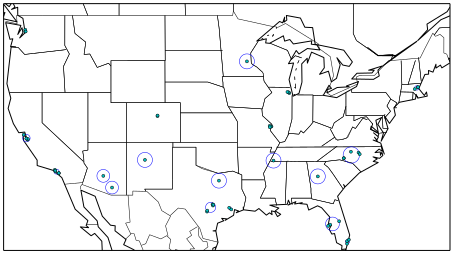
\includegraphics[width=\columnwidth]{figure1.png}}
\caption{\textbf{Depiction of an ObjArray OA whose .x attribute is coupled to buffer B.}  Like any ndarray, OA stores its indexed data in a contiguous block of memory: OA{[}0{]}...OA{[}N{]}.  Since OA has dtype=object, this data consists of pointers to the Python objects arrayed \textquotedbl{}within\textquotedbl{} OA:  Obj0, Obj1, ... ObjN.  OA also has its own attribute OA.x, which is a view of the entire buffer B.  During coupling, each arrayed object's .x attribute is made to be a property that provides a view of the corresponding portion of the buffer.  When an object's .x property is read, the corresponding buffer content is returned, and when that .x property is set to a new value, the new value is stored in the buffer.  Hence any changes to the buffer automatically appear as changes to object attributes and vice versa.}
\end{figure*}

Manual coupling to an existing array is allowed via \texttt{OA.couple\_to\_array(attr\_name, A)}.   This can be especially useful if you already have the values that you want for an attribute, especially one that doesn't exist yet in some or all of the objects, and/or if you want to ensure that the buffer for some \texttt{OA.x} will be located contiguously in memory with some other data, e.g., the buffer for some other \texttt{OA.y}, as such contiguity can be useful for some NumPy operations. For this latter usage, you would typically first allocate a double-sized buffer, then manually couple half of it to \texttt{'x'} and the other half to \texttt{'y'}.

Each attribute of each object can be coupled to only one buffer at a time!  To be coupled to a buffer, an object's attribute would need to store its value contiguously to those of the other objects in the same ObjArray, and that is (typically) incompatible with also storing its value contiguously to those of other objects in some other ObjArray. It is fine to have the same object be a member of multiple ObjArrays, but, for each attribute, no more than one of those ObjArrays should be coupled.  Best practice will usually be, for each attribute, to find the one array of objects you'll most often want to do vectorized NumPy operations on (or on slices from it) and couple that array, and then use ad hoc operations to read from or write to any other ObjArrays involving those same objects.

Coupling an object's attribute to a buffer creates a property with the same name in that object's class. (It would have been ideal to give this property just to the arrayed objects themselves, but alas one constraint of the Python language is that properties must be defined for classes.) This property is needed to ensure that attempts to set a coupled attribute instance won't break the coupling (when an object's attribute is assigned a new value, that new value should be put into the buffer, not displace the object's view of that subbuffer), and to allow attribute retrieval to yield a scalar value (rather than a tiny subarray containing just the scalar, which is technically what scalar attributes actually get coupled to). This new property will attempt to be as invisible as possible.  However, this precludes coupling \textquotedbl{}attributes\textquotedbl{} that were actually properties already. Typically you wouldn't want to do this anyway, because properties are useful for redirecting attempts to get/set them to third parties, whereas the point of coupling is instead to redirect such attempts to the buffer.  Also, the main advantage of coupling is that fast NumPy operations can alter the buffer and thereby effectively alter object attributes without needing to call anything like a \texttt{\_\_set\_\_} method for each object, whereas settable properties are intended to call a \texttt{\_\_set\_\_} method whenever an object's property is set to a new value, which would be so slow as to defeat the purpose of coupling.

Coupled buffers experience no slowdown at all for NumPy operations on the buffers, which are usually the operations for which speed is most crucial (goal N1).  Coupling may cause slight slowdown accessing or changing attributes from the object side though, because these operations are redirected to the relevant portion of the buffer.  This slowdown might be significant by NumPy standards, but not by the standards usually applicable for Python code that operates on objects one at a time.

\subsection{5.  The perils of dark magic and a vision of the future.%
  \label{the-perils-of-dark-magic-and-a-vision-of-the-future}%
}


I have implemented everything described above in my ObjArray package (available at \texttt{www.justin-fisher.com/research/objarray/}).  As far as I can tell it works fine, though it is freely distributed \textquotedbl{}as is\textquotedbl{} under a liberal BSD license.

My implementation is in pure Python 3.5, with use of NumPy iterators.  This provides a positive \textquotedbl{}proof of concept\textquotedbl{} showing that the eight goals described above can all be met.  This proof of concept is already quite useful for many purposes.  However, performance probably could be further optimized, perhaps by streamlining my Python code, or especially by re-implementing my inner loops in C to interface more directly with the inner workings of NumPy.  My code is profusely commented, so it should be fairly straightforward for other developers to modify as they please (though I would appreciate being informed of any bug-fixes or improvements that might be of use to me or others).

I have taken care to ensure that the \textquotedbl{}magic methods\textquotedbl{} ObjArray uses won't be too intrusive and won't do anything much different from what one would intuitively expect they should do.  However, such \textquotedbl{}dark magic\textquotedbl{} can come with real costs, potentially hiding unexpectedly complex behavior underneath misleadingly simple syntax, which sometimes makes bugs very hard to trace.  It's quite possible that I have not yet foreseen all the problematic interactions between the various hidden properties my dark magic required and the many scenarios of use to which ObjArrays might be put.  It will probably take public discussion and widespread testing to identify all these problematic interactions, and to find good remedies (or at least clear cautionary warnings) for them.

The ideal destination for my ObjArray package would be to have a future version of it be adopted as an optional subpackage within NumPy itself (e.g., as \texttt{numpy.objarray}).  I suppose it could be incorporated pretty much as is, and would likely be fairly useful to many users already as a much more convenient way to make good use of NumPy arrays with dtype=object.  It might be sensible, though, to have this undergo public discussion first, and/or for developers who better understand the under-the-hood workings of NumPy to optimize my inner loops in C.

Still, my proof of concept already works well enough to be tremendously useful in generating code that is simple, clean, fast, intuitive and beautiful.  This demonstrates that the rewards to be gained through my \textquotedbl{}dark magic\textquotedbl{} very likely will be worth the costs.  Of course, that's what practitioners of dark magic always say.
\end{document}
